\section{Results}
\subsection{Test of the voronoi tessellation}
Even thought the voronoi tessellation is performed in the 3D space, an example of implementation for two agents in the 2D plane is here presented in \autoref{fig:voronoi_example} because more understendable. The communication ranges are $R_{c1}=2.2, R_{c2}=0.55$ and a coverage factor of $\kappa=3$ has been used.  Here three different cases are reported: A) agents with point dimensions and $s_{max}=0$ (i.e. analogous to the continuous time implementation of the algorithm) and perfect localizations, B) finite physical encumbrance $\delta_1=0.25$, $\delta_2=0.15$, finite space $s_{max,1}=1$, $s_{max,2}=0.35$ and perfect localization, C) finite physical encumbrance, finite velocity and uncertainty in localization $\sigma_{1}^1=\sigma_{2}^2=0.05^2 \text{\textit{I}}_3, \sigma_{1}^2=0.1^2 \text{\textit{I}}_3, \sigma_{2}^1=0 \text{\textit{I}}_3$.
\begin{figure}[htb]
\centering
    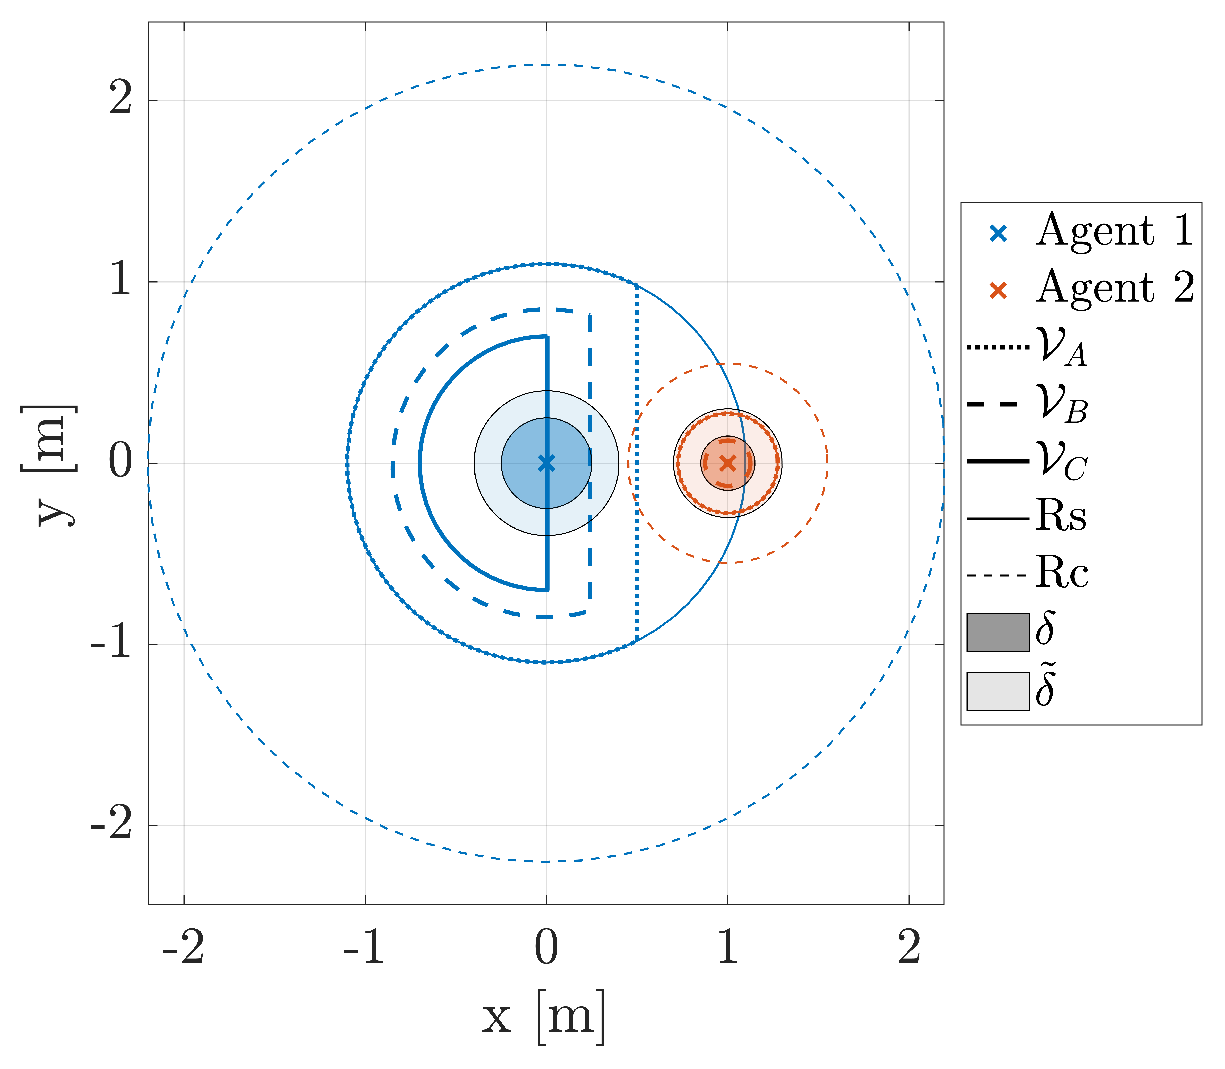
\includegraphics[width=0.7\columnwidth]{images/fig_voronoi_example.eps}
    \caption{Example of the voronoi tessellation for two agents in the plane. $\mathcal{V}_A$ is build considering only the position of the agents, $\mathcal{V}_B$ considers finite dimensions and velocities while $\mathcal{V}_C$ considers also the uncertainties }
    \label{fig:voronoi_example}
\end{figure}
In case A, agent \textit{1} sees \textit{2} inside its communication range and sets its cell limit at half their distance; chute \textit{2} does not see \textit{1} and so its cell becomes the whole circle with radius $R_{c2}$. In case B, agents \textit{1} and \textit{2} in one time step can reach the limit of the cell, so they have to shrink their old cells of $\delta_1$ and $\delta_2$. The voronoi limit of agent \textit{2} moves inside the encumbrance of the chute itself. In case C, on top of what already happened in case B, \textit{1} further shrinks its limits so that in the direction between \textit{1} and \textit{2} the limit goes above \textit{1}. Meanwhile \textit{2} increases its encumbrance, reducing its voronoi limit more than the dimension of the previous area leading the final cell to be a point. In that final condition, \textit{1} cannot move towards while \textit{2}, while \textit{2} cannot move at all.

\subsection{Example of a complete swar trajectory}
\autoref{fig:3D_traj} shows the trajectory followed by 13 parachutes falling from an initial position located around the point $p_0=[500, 500, 1000]$ and falling twords $[0, 0, 0]$, while \autoref{fig:state} shows the time evolution of states and control inputs for one of the falling parachutes. The wind noise has been set to 3 $\left[\si{\meter\per\second}\right]$ in every directions.\\
\begin{figure}[h]
    \centering
    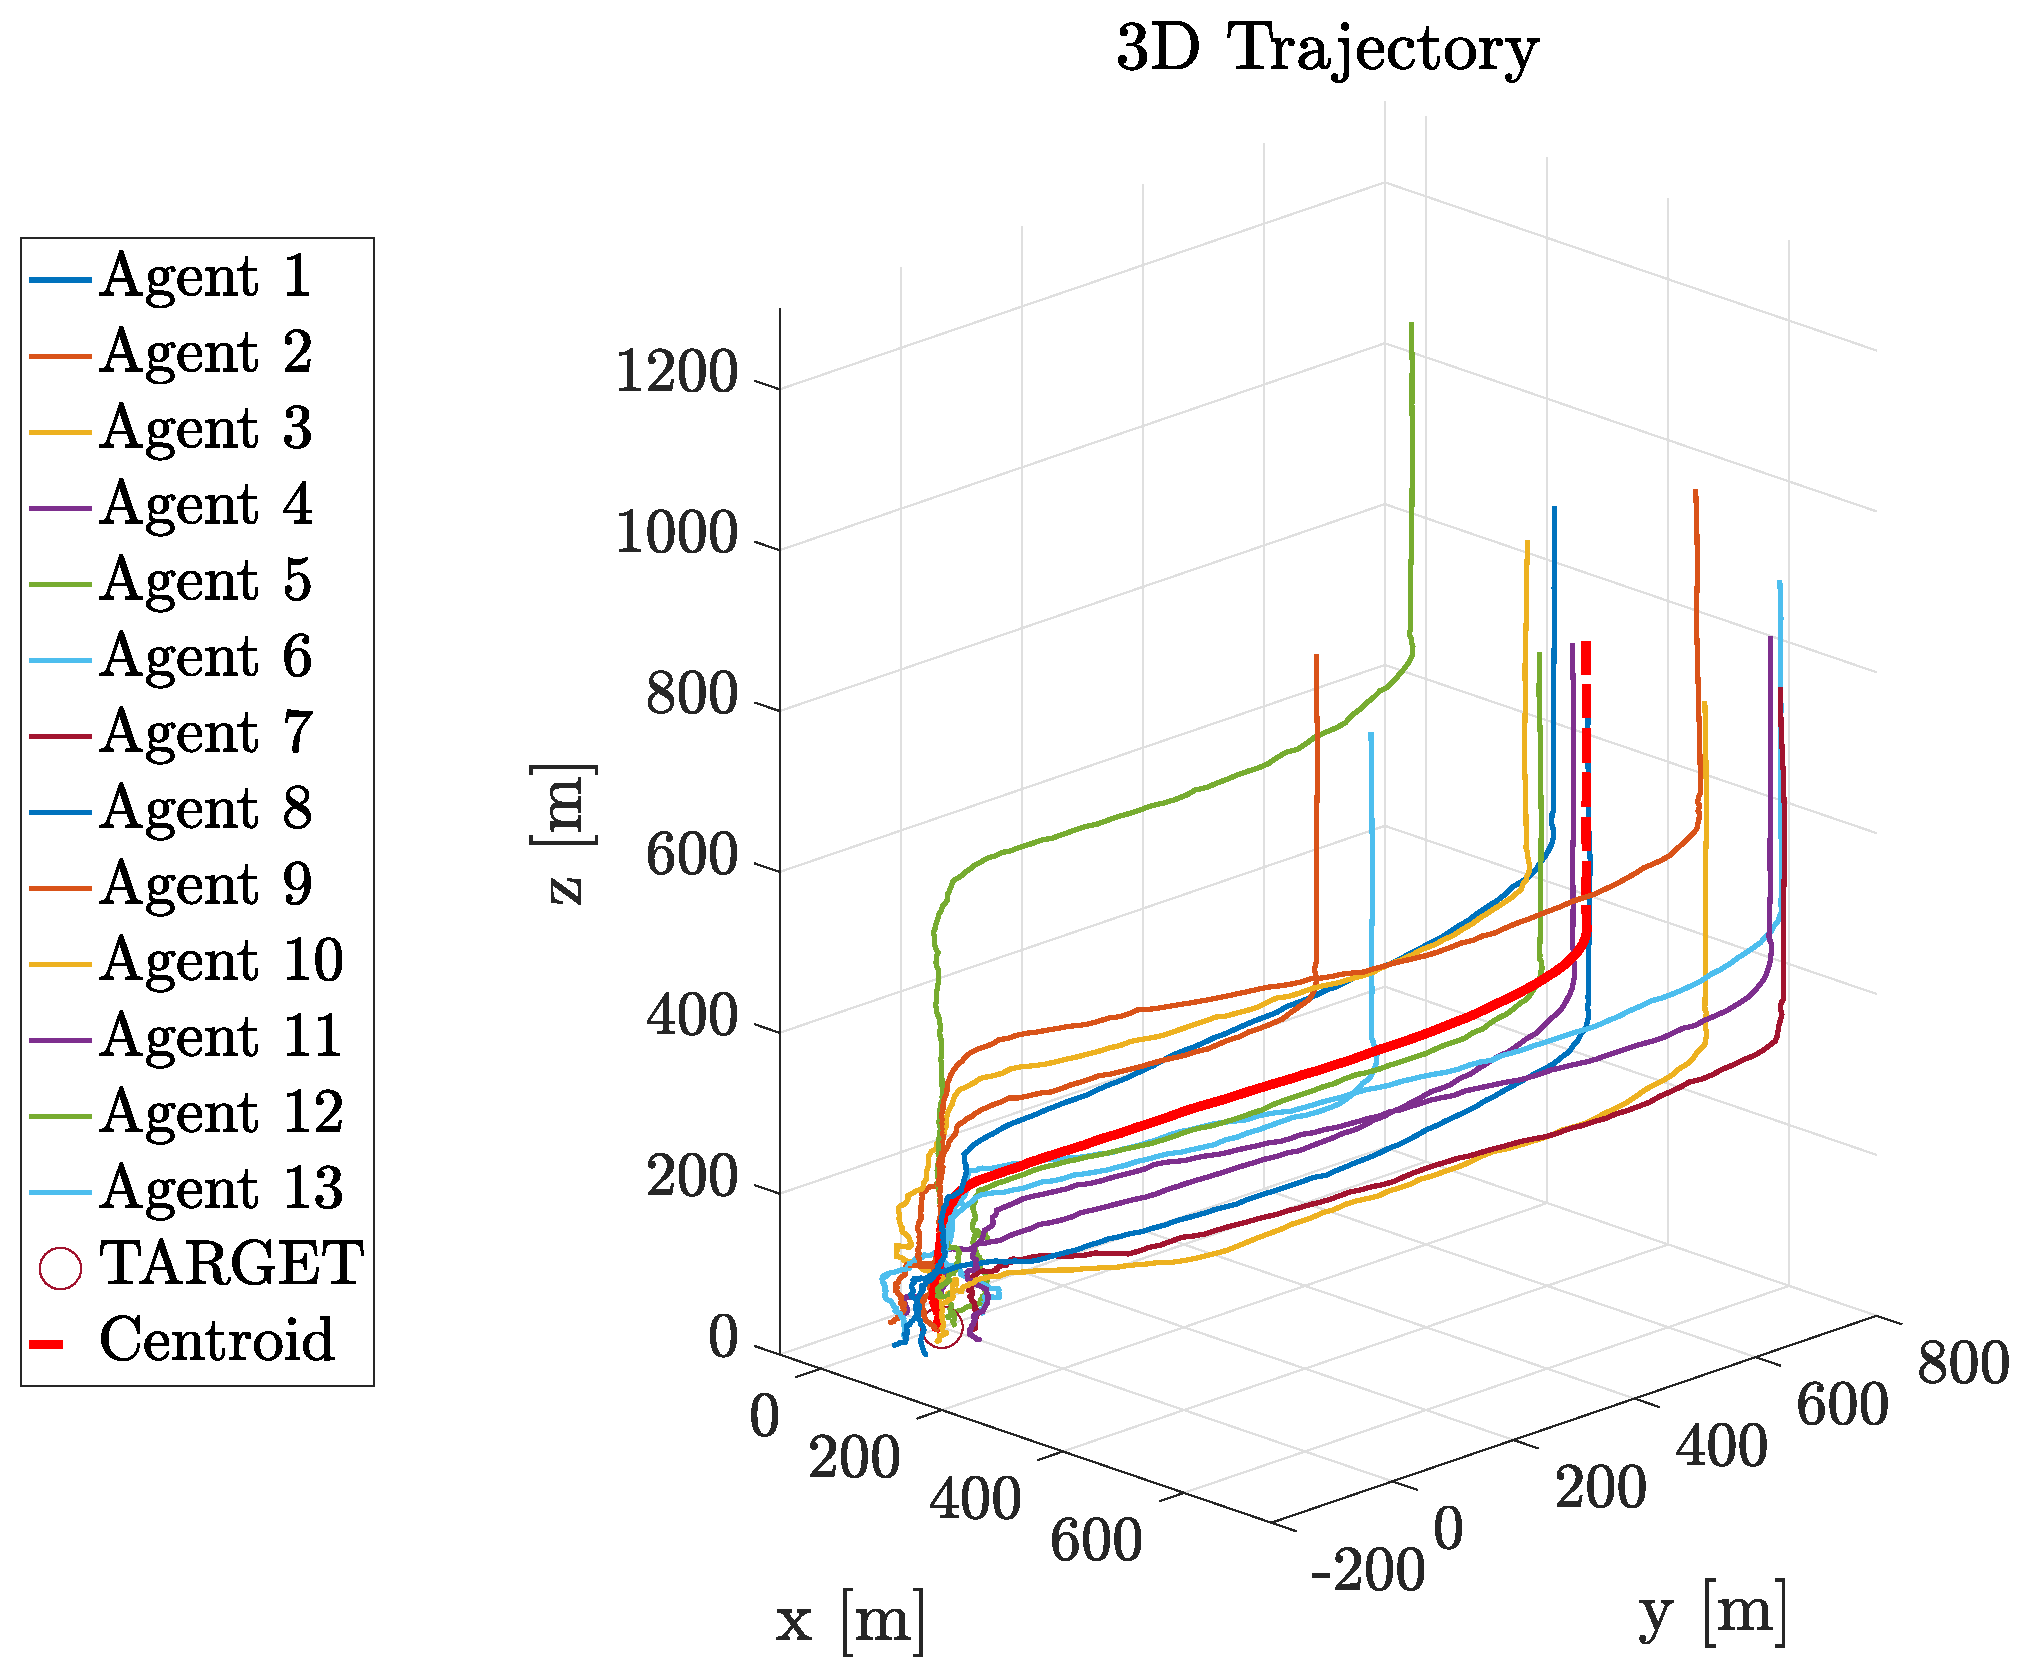
\includegraphics[width=\columnwidth]{images/fig_3D.eps}
    \caption{3D trajectory with 13 parachutes and all probabilities set to 1.}
    \label{fig:3D_traj}
\end{figure}
\begin{figure}[h]
    \centering
    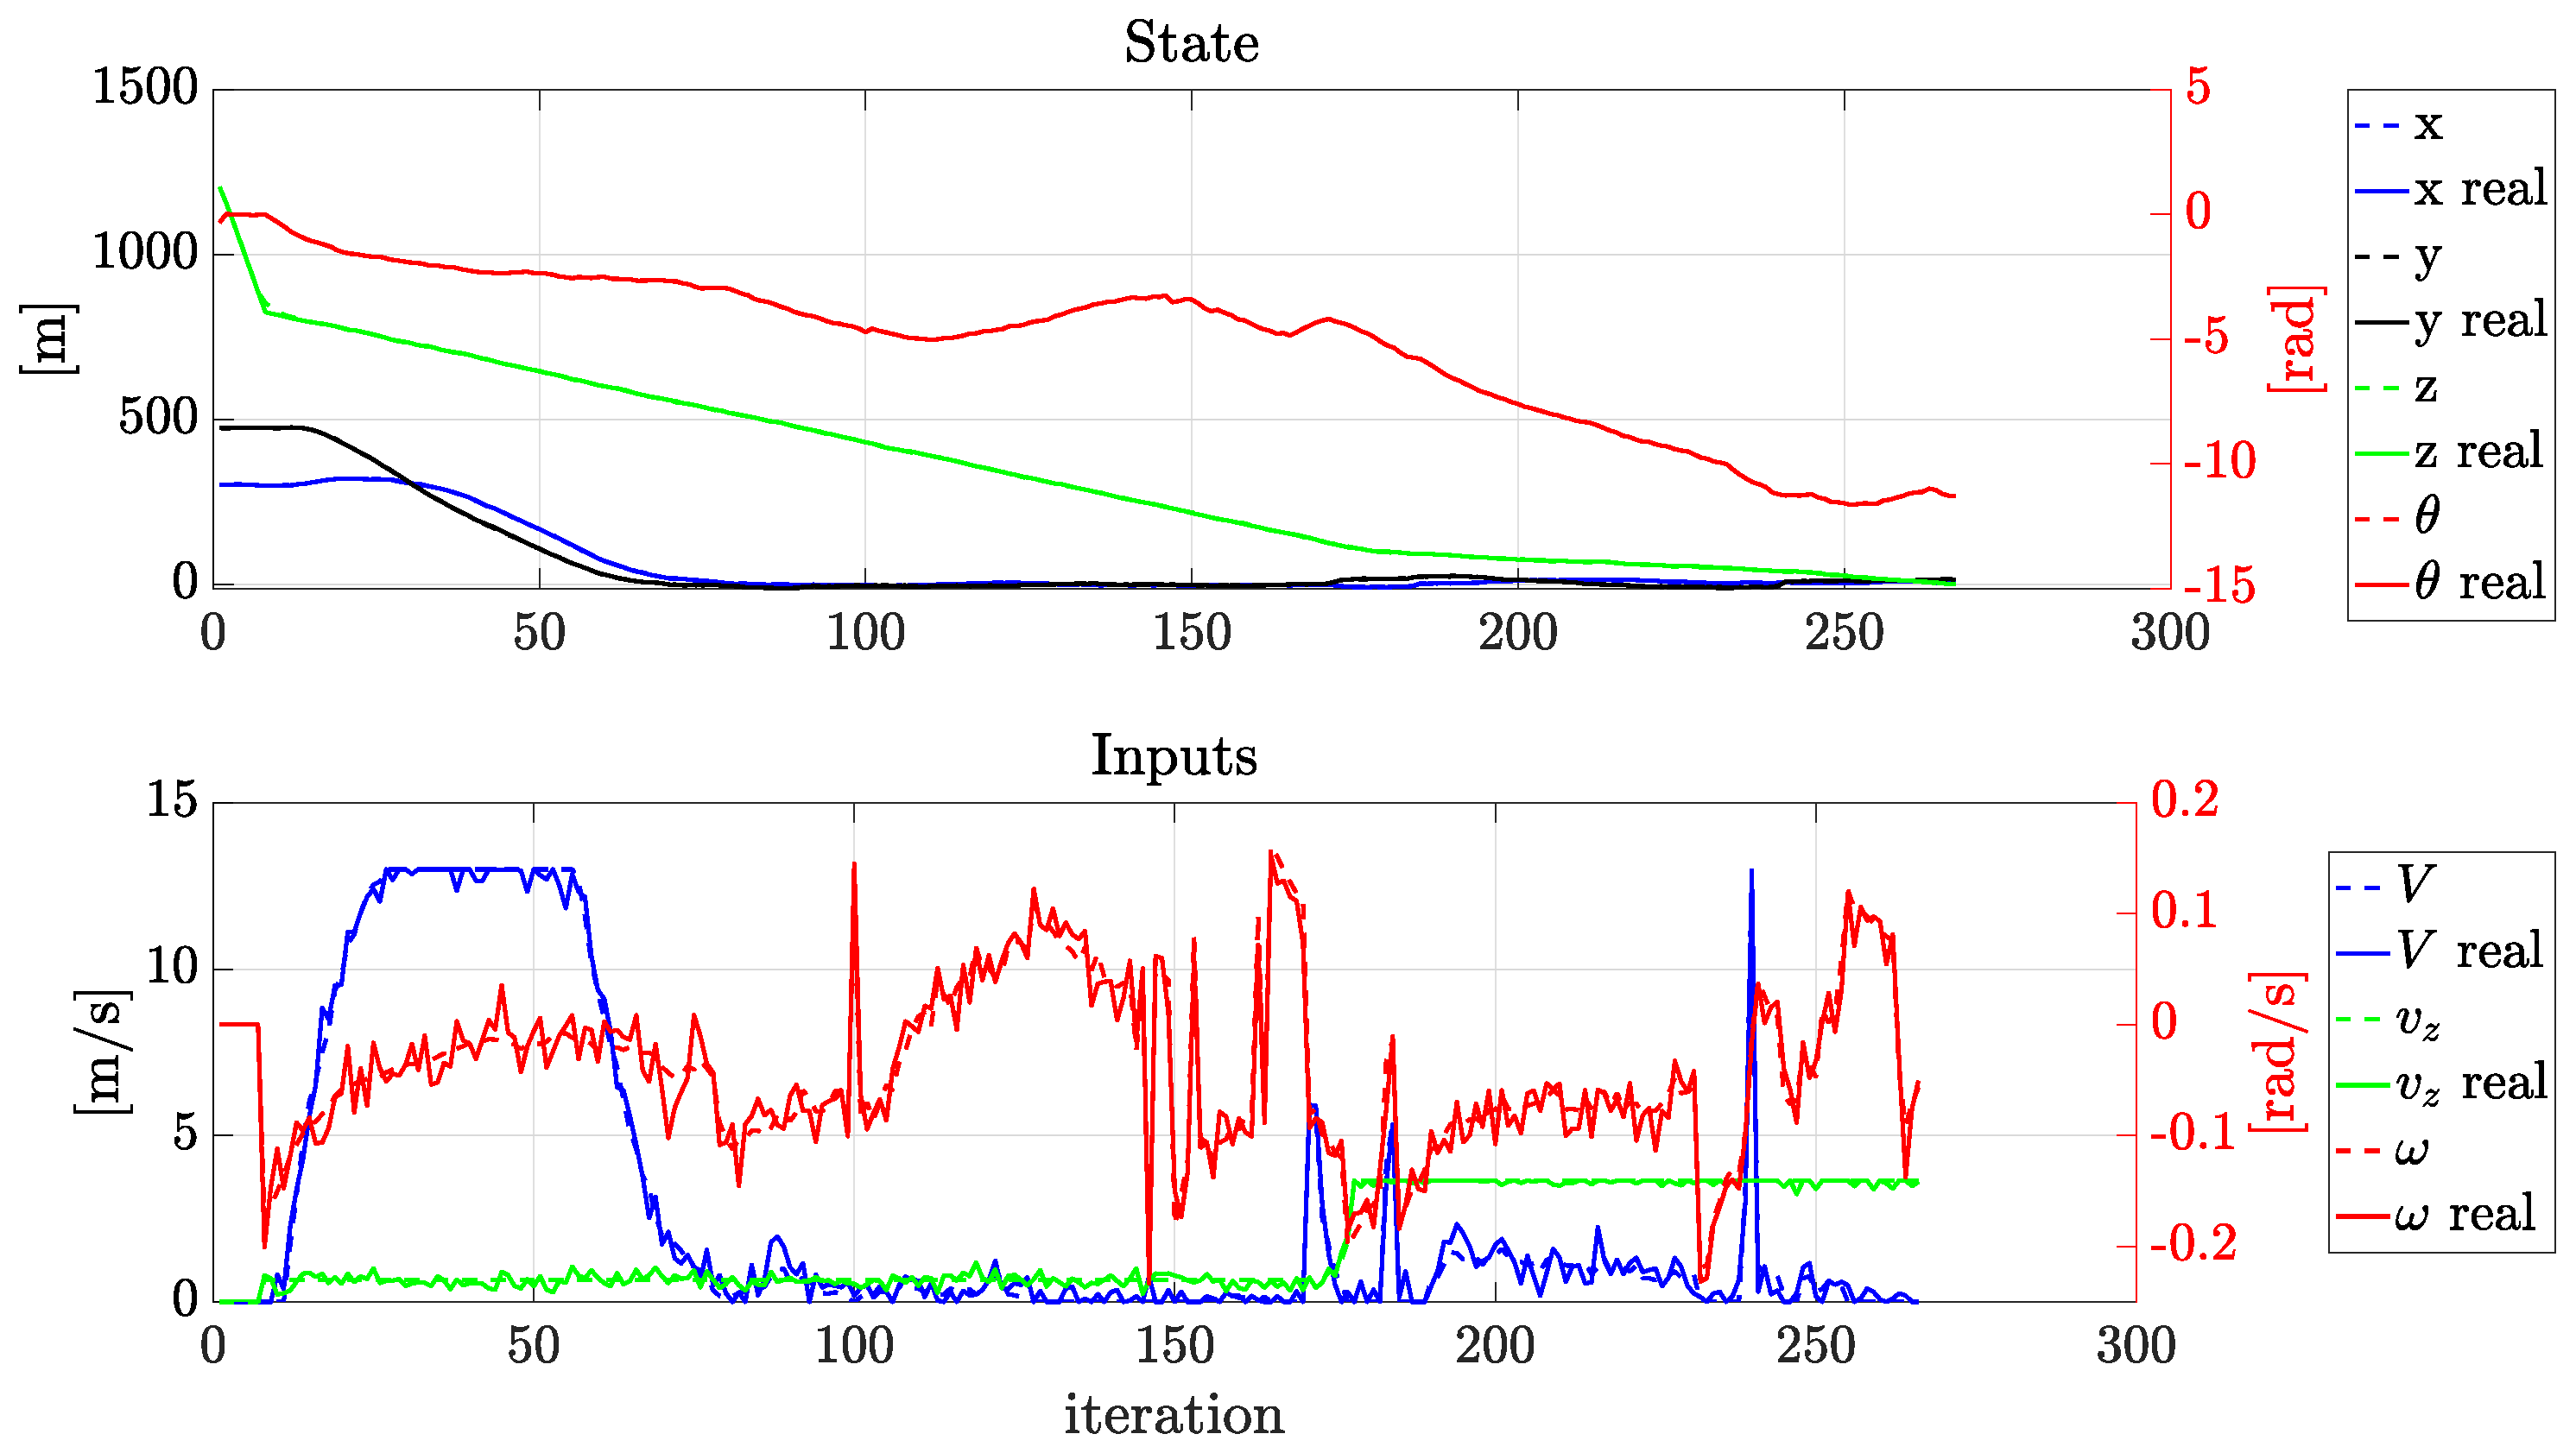
\includegraphics[width=\columnwidth]{images/fig_1.eps}
    \caption{States and inputs behaviour of agent 12.}
    \label{fig:state}
\end{figure}
It could be seen that the centroid (red dashed line of \autoref{fig:3D_traj}) reaches correctly the target, while the parachutes fall around it without any collision.\\
For what concerns the inputs, it may be noticed that in the initial free fallin part, there is no actuation, while in the final part the control on the z axis is saturated to reduce the speed before the contact with ground. Also the forwar velocity is saturated in the central part, where the agent is moving towrds the target. 

\subsection{Distributed WLS}
\autoref{fig:ab_IK} represents the standard deviation of the localization error commited by agent 7 in the localization of the others before and after the distributed of information via WLS algorithm, in the three directions. It must be noted that \textit{before WLS} considers the localization at the time steps when the relative distance measurement is performed or when the dynamic of the other is propagated through the model. On the other hand, \textit{after WLS} considers the result of the consensus algorith, so in that time instant the localization can be also based only on the information shared by the network with the considered one.
\begin{figure}[h]
    \centering
    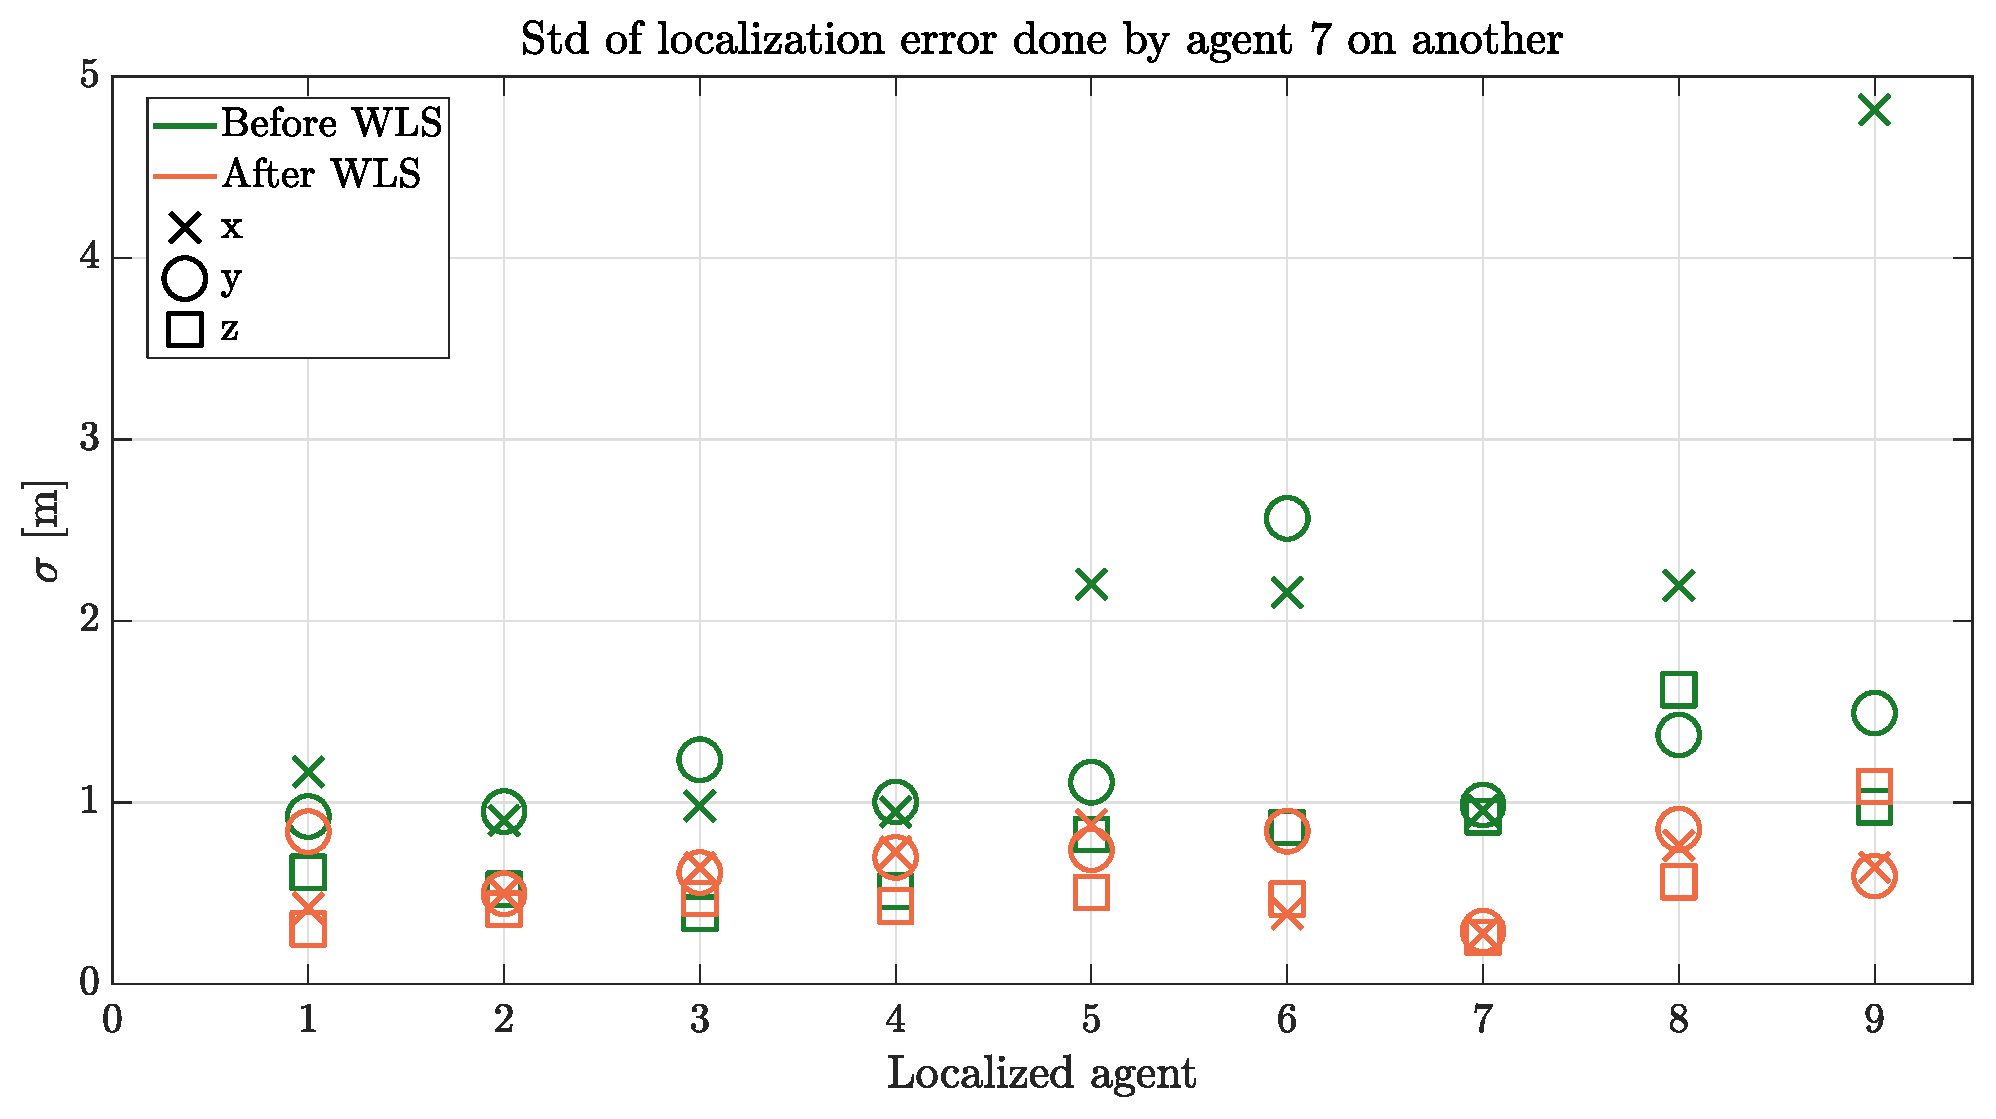
\includegraphics[width=\columnwidth]{images/mdl2_9chutes_be_wls.eps}
    \caption{Standard deviation of the error made by the parachute 7 on the localization of the others.}
    \label{fig:ab_IK}
\end{figure}

\subsection{Effect of the Inverse Kinematics}
In order to test the effectiveness of the IK in the navigation, a comparative test as been done. In particular, a given number of parachutes has been driven with and without the use of the IK. The initial conditions of the two cases are the same for a given round and more round have been run. No uncertainties and noises have been introduced in order to highlight the effect of the navigation only. Finally, the distance between the centroid and the target has been computed alongside with the Root Mean Square (RMS) of the agent to target distance. The mean results among multiple rounds are collected in \autoref{tab:IK_comparison}.
\begin{table}[]
\scriptsize
  \caption{Comparison between the use of IK or not}
  \centering
  \begin{tabular}{ccccc|cccc}
  \hline
  & \multicolumn{4}{c}{Linear} & \multicolumn{4}{c}{Non-linear}\\
  \multicolumn{1}{c}{\#} & \multicolumn{2}{c}{Dist.} & \multicolumn{2}{c}{RMS} & \multicolumn{2}{c}{Dist.} & \multicolumn{2}{c}{RMS}\\
  \multicolumn{1}{l}{}  & IK & No IK & IK & No IK & IK & No IK & IK & No IK \\ \hline
  1   & 2.99 & 0.01 & 2.99 & 0.01 & 3.00 & 0.02 & 3.00 & 0.02  \\
  3   & 6.21 & 3.05 & 25.36 & 33.34 & 7.72 & 4.42 & 25.36 & 27.74 \\
  5   & 4.32 & 6.13 & 29.41 & 38.76 & 6.86 & 5.61 & 32.84 & 39.83 \\
  7   & 3.07 & 4.86 & 35.20 & 41.88 & 6.30 & 4.57 & 32.62 & 47.31 \\
  9   & 5.12 & 5.47 & 37.56 & 49.35 & 7.21 & 8.64 & 41.49 & 48.43 \\
  11  & 2.31 & 2.53 & 43.18 & 53.43 & 8.83 & 5.90 & 43.44 & 55.80 \\
  13  & 4.70 & 3.47 & 46.37 & 58.23 & 3.42 & 7.52 & 46.91 & 57.78 \\
  \hline
  \end{tabular}
  \label{tab:IK_comparison}
\end{table}


It could be seen that the IK approach reduces the dispersion of the chutes around the target, thanks to the postural task, for both models, while the distance of the global centroid from the target seems independent of the choice, except in the case of only one parachute. However, since it may be preferable to have all the parachutes as near as possible to the target, the RMS is a better estimator of the success of the task. Hence, the use of the IK is preferable and all the next studies are done using this technique.
\subsection{Effect of the probabilities}
A parametric study has been conducted changing the probability of having the GPS measurement, the relative measurement between chutes. In this simulation 9 parachutes of the nonlinear type are considered, the initial falling part and the final deceleration are removed, while the noises are considered. In each of the test, one of the probabilities has been changed while the other has been kept constant to 100\%. After the simulation, the standard deviation of the localization error in the 3 directions has been computed both for the self localization in \autoref{fig:self_loc} and on the others in \autoref{fig:other_loc}. For the latter case the mean of the error on all the others is reported.
\begin{figure}[h]
    \centering
    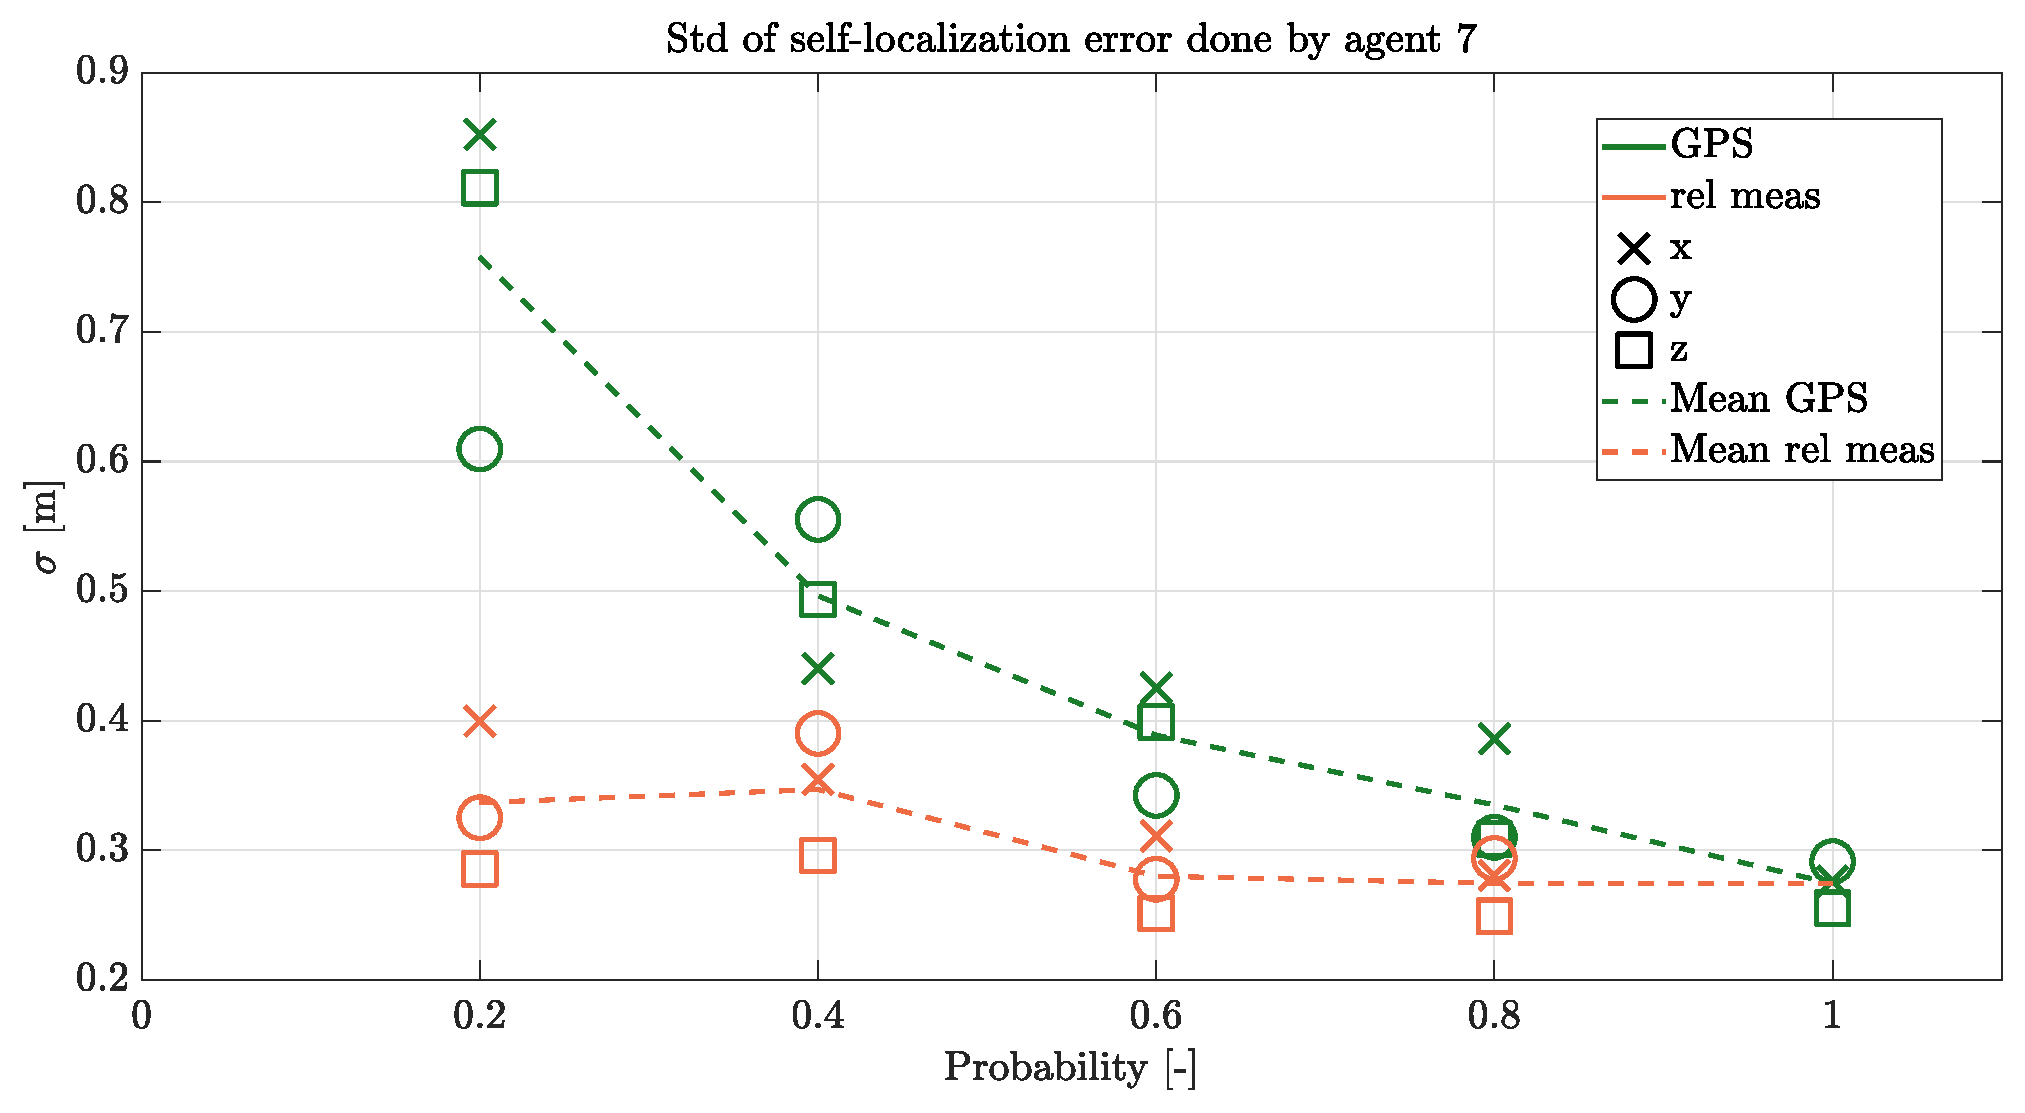
\includegraphics[width=\columnwidth]{images/mdl2_9chutes_parametric_beforeconsensus.eps}
    \caption{Standard deviation of the localization error made by the parachute 7 on itself at different values of GPS and relative measurements probabilities.}
    \label{fig:self_loc}
\end{figure}
\begin{figure}[h]
    \centering
    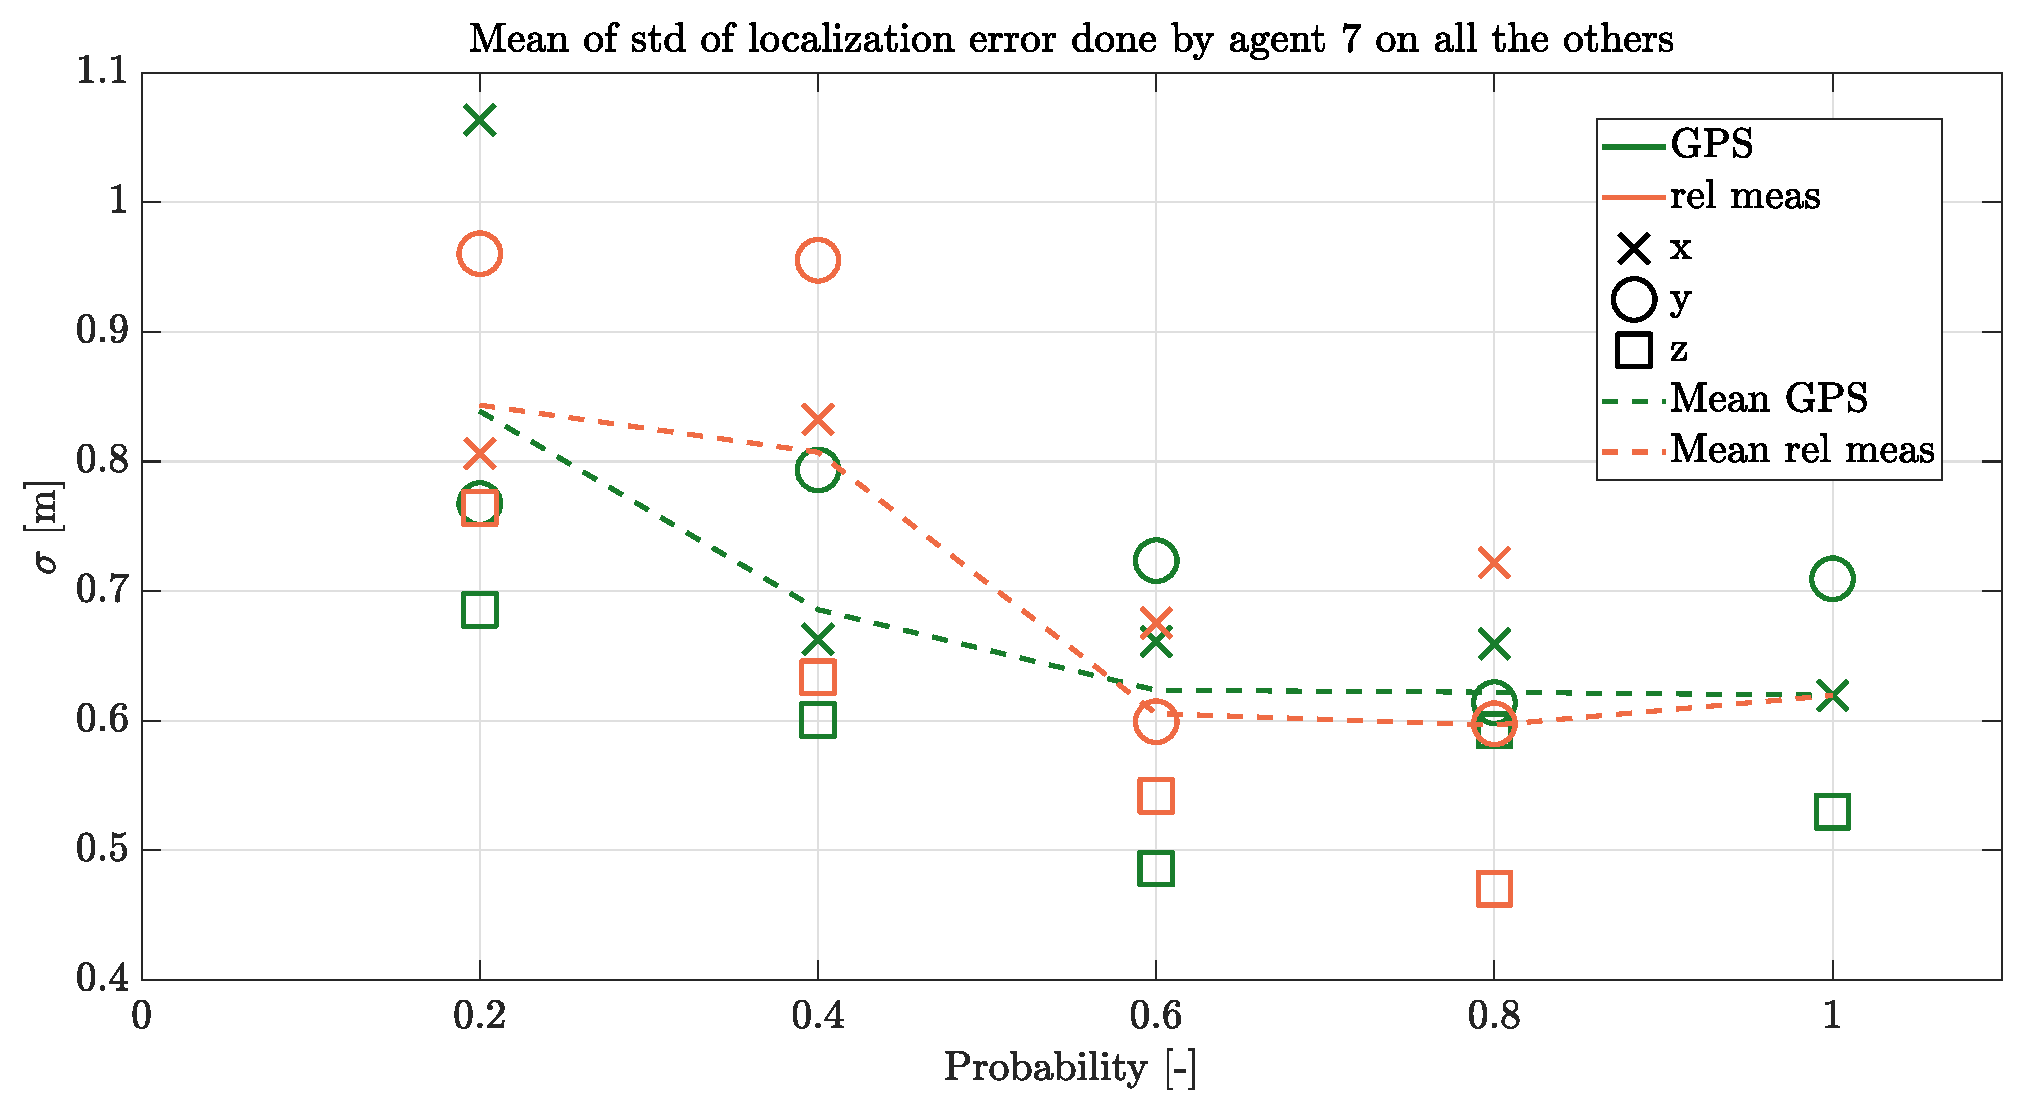
\includegraphics[width=\columnwidth]{images/mdl2_9chutes_parametric_loc_others.eps}
    \caption{Standard deviation of the localization error made by the parachute 7 on the others parachutes at different values of GPS and relative measurements probabilities.}
    \label{fig:other_loc}
\end{figure}
From the graph, it can be seen that the self localization error is more affected by the GPS probability rather than the by the relative measurement. This may also explain why it seems that after all the probability of performing the relative measuerement is not so important. On the other hand the two effects are more combined in the localization errors made on the others \textcolor{red}{Scrivere qulche commento i più}